% =============================================================================
% did-two-period.tex — Two-period difference-in-differences visualization
%
% Shows: treated and control groups over two periods. Counterfactual treated
% path (parallel trends assumption) drawn dashed. DiD estimate is the gap
% between observed and counterfactual treated at t = 1.
%
% Compiles standalone via: xelatex did-two-period.tex
% =============================================================================

\documentclass[border=4pt]{standalone}
\usepackage{tikz}
\usetikzlibrary{arrows.meta}

\definecolor{treated}{HTML}{B23A48}
\definecolor{control}{HTML}{3A6EA5}
\definecolor{counterf}{HTML}{8A8A8A}
\definecolor{axes}{HTML}{1A1A1A}

% -----------------------------------------------------------------------------
% Diagram: 2-period DiD with observed paths (solid) and counterfactual (dashed).
% Coordinates (x-axis = period, y-axis = outcome):
%   control0 at (0, 1.0)   control1 at (4, 1.4)   -- control path
%   treated0 at (0, 2.0)   treated1 at (4, 3.8)   -- observed treated
%   counterf at (4, 2.4)                          -- counterfactual treated
% Nothing is scaled. DiD = treated1.y - counterf.y = 3.8 - 2.4 = 1.4.
% -----------------------------------------------------------------------------

\begin{document}
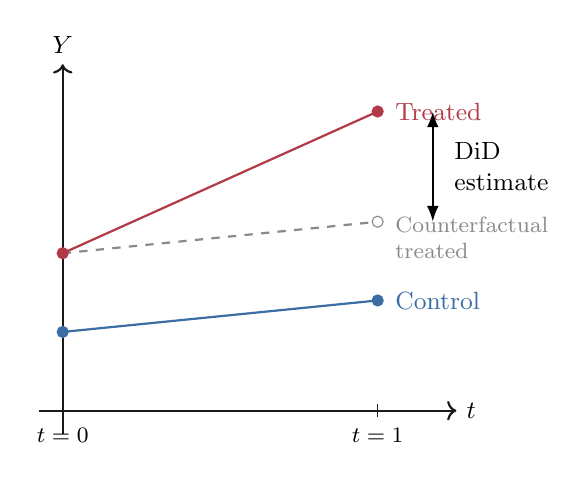
\begin{tikzpicture}
  % Axes
  \draw[->, thick, draw=axes] (-0.3, 0) -- (5, 0) node[right] {\small $t$};
  \draw[->, thick, draw=axes] (0, -0.3) -- (0, 4.4) node[above] {\small $Y$};
  \draw[draw=axes] (4, -0.08) -- (4, 0.08);
  \node[below] at (0, -0.1) {\footnotesize $t=0$};
  \node[below] at (4, -0.1) {\footnotesize $t=1$};

  % Control path (solid)
  \draw[thick, draw=control] (0, 1.0) -- (4, 1.4);
  \filldraw[control] (0, 1.0) circle (2pt);
  \filldraw[control] (4, 1.4) circle (2pt);
  \node[right, control, font=\small] at (4.1, 1.4) {Control};

  % Counterfactual treated (dashed)
  \draw[thick, dashed, draw=counterf] (0, 2.0) -- (4, 2.4);
  \draw[counterf, fill=white] (4, 2.4) circle (2pt);
  \node[right, counterf, font=\footnotesize, align=left] at (4.1, 2.2)
    {Counterfactual\\treated};

  % Observed treated (solid)
  \draw[thick, draw=treated] (0, 2.0) -- (4, 3.8);
  \filldraw[treated] (0, 2.0) circle (2pt);
  \filldraw[treated] (4, 3.8) circle (2pt);
  \node[right, treated, font=\small] at (4.1, 3.8) {Treated};

  % DiD bracket at t=1
  \draw[thick, {Latex[length=2mm]}-{Latex[length=2mm]}] (4.7, 2.4) -- (4.7, 3.8);
  \node[right, font=\small, align=left] at (4.85, 3.1) {DiD\\estimate};
\end{tikzpicture}
\end{document}
